227. \begin{figure}[ht!]
\center{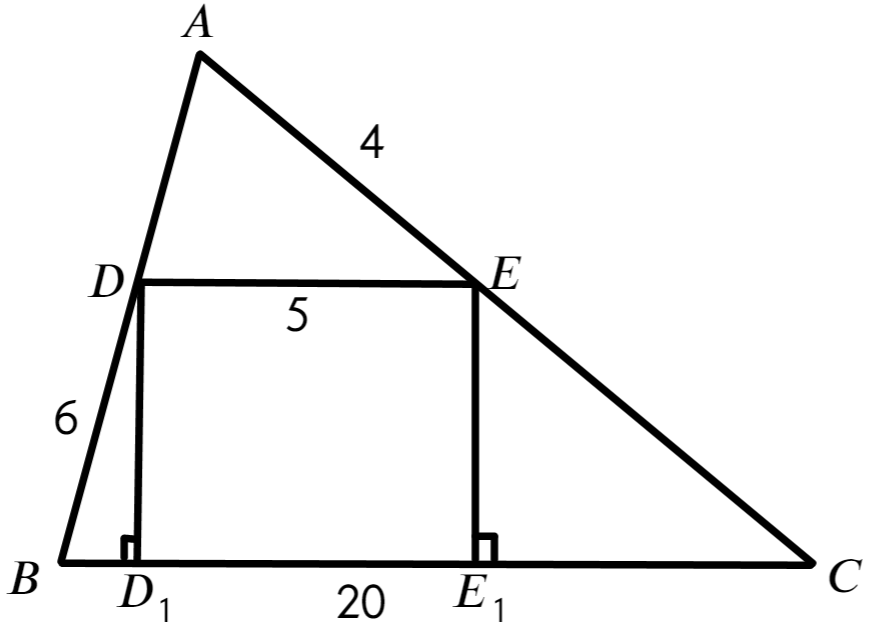
\includegraphics[scale=0.35]{g8-227.png}}
\end{figure}\\
Треугольники $ABC$ и $ADE$ подобны по двум углам (соответственным при параллельных прямых $BC$ и $DE$). Коэффициент подобия равен $\cfrac{BC}{DE}=\cfrac{20}{5}=4.$ Значит, $AC=4AE=4\cdot4=16,$ откуда $EC=16-4=12.$ Опустим в трапеции высоты $DD_1$ и $EE_1.$ Пусть $BD_1=x,$ тогда $E_1C=20-x-5=15-x.$ Выразив квадрат высоты трапеции по теореме Пифагора для треугольников $BDD_1$ и $CEE_1,$ получим равенства $h^2=36-x^2=144-(15-x)^2,$ поэтому $36-x^2=144-225+30x-x^2,\ 30x=117,\ x=\cfrac{39}{10}.$ Тогда $h^2=36-\left(\cfrac{39}{10}
ight)^2=\cfrac{2079}{100},\ h=\cfrac{3\sqrt{231}}{10}.$ Таким образом, $P=6+5+12+20=43,\ S=\cfrac{3\sqrt{231}}{10}\cdot\cfrac{5+20}{2}=\cfrac{15\sqrt{231}}{4}.$\\
